\documentclass[12pt,a4paper]{article}
\usepackage[T1]{fontenc}
\usepackage[utf8]{inputenc}
\usepackage{lmodern,amsmath,amssymb,amsthm,mathtools}
\usepackage[a4paper,margin=25mm]{geometry}
\usepackage{microtype,booktabs,array,enumitem}
\usepackage{tikz}
\usetikzlibrary{arrows.meta,positioning}
\usepackage[colorlinks=true,linkcolor=blue!50!black,urlcolor=blue!50!black,citecolor=blue!50!black]{hyperref}
\setlength{\emergencystretch}{3em}
\setlength{\parskip}{.25em}
\setlist{nosep}
\newtheorem{theorem}{Theorem}
\newtheorem{lemma}[theorem]{Lemma}
\newtheorem{proposition}[theorem]{Proposition}
\newtheorem{corollary}[theorem]{Corollary}
\theoremstyle{remark}
\newtheorem{remark}[theorem]{Remark}
\newcommand{\HV}{\operatorname{HV}}
\newcommand{\Mag}{\operatorname{Mag}}
\newcommand{\1}{\mathbf1}
\newcommand{\wtO}{\widetilde O}
\newcommand{\PairSum}{\operatorname{PairSum}}
\newcommand{\SumOut}{\operatorname{SumOut}}
\newcommand{\Push}{\operatorname{Push}}
\hypersetup{pdftitle={A Numerical 2+2 Form of Chan's Four-Dimensional Hypervolume Algorithm},
pdfsubject={Finite weighted chains, numerical pair elimination, and a proved n to the 4/3 recurrence}}
\title{A Numerical $2+2$ Form of Chan's\\Four-Dimensional Hypervolume Algorithm\\[.5em]
\large Finite weighted chains, pairwise summation, and an explicit recursion}
\author{Research working report}
\date{4 October 2026}
\begin{document}
\maketitle

\begin{abstract}
We give an exact numerical formulation of four-dimensional anchored
hypervolume and dominated-set $\ell_1$ magnitude with
$\wtO(n^{4/3})$ arithmetic complexity. The exponent is Chan's;
the purpose is a simpler implementation and a transparent recurrence.
Each coordinate is replaced by a finite ordered list of cells carrying
numerical masses. The state consists only of numerical unary arrays,
integer monotone cutoff arrays, and scalar coefficients. Eliminating a
variable uses a prefix sum and deterministic choices of its active lower
and upper bounds. Compression stores block \emph{masses}, so it needs
neither symbolic integration nor average densities or division by cell
measure. Opposite monotonicity directions remain separate, avoiding
finite-run inversion and special endpoint decorations.

Two coordinate eliminations form the numerical pair operation. Two pairs
of binary cuts form a geometric round: at most sixteen descendants have
one eighth of the parent's weighted face complexity. Locally chosen
blocks give $O(\log\log n)$ compression generations; a constant raw
emission factor per generation is consequently only polylogarithmic.
This explicitly accounts for representation growth. A standalone Python
prototype and exact verification accompany the report. The result is an
arithmetic-complexity formulation, not a claim of competitive floating-point
performance or an improvement over Chan's exponent.
\end{abstract}

\newpage
\tableofcontents
\newpage

\section{The target and the simplification}
For a finite set $P\subset\mathbb R_{\ge0}^4$, write
\[
 D(P)=\bigcup_{p\in P}\prod_{i=1}^4[0,p_i].
\]
The two requested quantities are
\[
 \HV_4(P)=\lambda_4(D(P)),\qquad
 \Mag(D(P))=
 \Bigl(\bigotimes_{i=1}^4(\delta_0+\tfrac12\lambda)\Bigr)(D(P)).
\]
The second equality is the product-measure form of the dominated-set
magnitude formula in Emmerich~\cite{emmerich}. Empty input has value zero
for both quantities. Zero coordinates are permitted and matter for magnitude.

Chan's orthant algorithm gives the $\wtO(n^{d/3})$ bound for fixed
$d\ge4$~\cite{chan}. Its essential ingredients are absorption of locally
one- and two-sided orthants, weighted geometric cuts, and periodic
compression. We retain these ingredients. The continuous function algebra
is replaced by finite tables and exact summation.

\begin{theorem}[Numerical four-dimensional formulation]\label{thm:main}
There is an algorithm for $\HV_4(P)$ and $\Mag(D(P))$ using
$O(n^{4/3}\log^c(n+2))$ arithmetic operations, for a fixed constant $c$.
Its operations are sorting, comparisons, integer-index searches, and
arithmetic on numerical arrays. It uses no symbolic integration or
numerical quadrature. It does not construct a four-dimensional product grid.
\end{theorem}

The proof includes representation growth and compression work, not just
the number of geometric leaves. Arithmetic operations have unit cost;
the theorem is not a bit-complexity or numerical-stability bound.
Here $\wtO$, or $O^*$ in the sense intended in the question, suppresses
polylogarithmic factors and fixed-dimensional constants.

The principal simplifications are these:
\begin{enumerate}
\item Store one mass for each one-dimensional cell, including the anchor.
\item Keep four monotonicity/comparison classes per coordinate pair.
\item Replace every one-dimensional antiderivative by an array prefix sum.
\item Compress by summing mass into blocks; do not reconstruct a density.
\item Allow polylogarithmically many terms and prove their total cost.
\end{enumerate}
The active-bound choices and compression itself remain necessary parts
of this construction. Merely deleting them would not preserve the proof.

\section{From product measure to finite weighted chains}\label{sec:cells}
On axis $i$, sort the distinct positive input coordinates:
\[
             0=c_{i,0}<c_{i,1}<\cdots<c_{i,m_i}.
\]
Use the cells
\[
 C_{i,0}=\{0\},\qquad
 C_{i,k}=(c_{i,k-1},c_{i,k}]\quad(1\le k\le m_i).
\]
For a measure $\alpha_i\delta_0+\beta_i\lambda$, give these cells masses
\begin{equation}
 a_i(0)=\alpha_i,\qquad
 a_i(k)=\beta_i(c_{i,k}-c_{i,k-1}).                 \label{eq:cellmass}
\end{equation}
Hypervolume uses $(\alpha_i,\beta_i)=(0,1)$; magnitude uses
$(1,\tfrac12)$. Keeping a zero-weight anchor cell for hypervolume is harmless
and lets both computations use identical code.

Let $r_i(p)$ be the coordinate rank of $p_i$, with rank zero at the anchor.
On a cell product, membership in $[0,p]$ is exactly
\[
                 k_i\le r_i(p)\quad\hbox{for every }i.
\]
Thus the original continuous measure is the finite weighted sum of these
membership indicators. Only the four \emph{axis lists} are constructed;
their Cartesian product is a specification, not an allocated array.

\begin{lemma}[Exact discretization]\label{lem:discrete}
Replacing each input corner by its four ranks and using
\eqref{eq:cellmass} preserves both requested values exactly. The total
axis-list length is at most $4(n+1)$, and construction costs $O(n\log n)$.
\end{lemma}
\begin{proof}
Every box-membership predicate is constant on each cell product. Product
measure assigns that cell the product of its four one-dimensional masses.
Summing over covered cells is therefore exact. Sorting and rank lookup
construct the one-dimensional lists in the stated time.
\end{proof}

All later computation uses indices. A feasible index interval $[L,U]$ is
empty precisely when $L>U$. In particular, the anchor interval $[0,0]$
is different from the empty interval $[0,-1]$. There are no open/closed
endpoint flags or infinite numerical values in the computational state.

For example, coordinates $0,2,5$ give magnitude masses
$(1,1,3/2)$. The prefix array is $(0,1,2,7/2)$.
The anchor has mass $1$, while indices $1,2$ together have mass $5/2$.

\section{The numerical state and its invariant}\label{sec:state}
Variables have finite ordered domains
$E_i=\{0,\ldots,s_i-1\}$. A term is
\begin{equation}
 T(k)=\gamma\prod_i a_i(k_i)
           \prod_{e}\1[k_{j_e}\mathrel{\bowtie_e}f_e(k_{i_e})],
 \qquad \bowtie_e\in\{\le,\ge\}.                 \label{eq:term}
\end{equation}
The coefficient $\gamma$ and arrays $a_i$ may be signed. Each cutoff
$f_e$ is an integer-valued monotone array. Endpoints $-1$ and $s_j$
encode empty rays when appropriate.

Order each pair so that $i<j$. Store at most four cutoff arrays per pair:
\[
 \begin{array}{c|cc}
       & f\text{ nondecreasing}&f\text{ nonincreasing}\\\hline
 k_j\le f(k_i)&\text{one slot}&\text{one slot}\\
 k_j\ge f(k_i)&\text{one slot}&\text{one slot}
 \end{array}
\]
Within the same slot, upper bounds merge by pointwise minimum and lower
bounds by pointwise maximum. These operations preserve the recorded
monotonicity. A constant cutoff can be absorbed into the target unary
array. Opposite monotonicity directions are \emph{not} merged.

This fixed four-slot rule is important. It keeps the class unchanged after
every compression; it does not merely bound a list whose permitted length
might grow at the next generation. No valley or zigzag inverse is needed.

For $p$ variables, a term has at most $4\binom p2$ pair conditions.
With $M=\sum_i s_i$, its storage is $O_p(M)$. All arrays can be dense
one-dimensional arrays; sparse step records are optional optimizations.
A state $F$ is a signed sum of $S$ such terms.

The geometric recursion also carries a cell
$\Gamma=\prod_i[\ell_i,u_i]$ of index ranges and a list $B$ of
unabsorbed rank corners. Its invariant is the numerical quantity
\begin{equation}
 U(F,B,\Gamma)=\sum_{k\in\Gamma}F(k)
                   \prod_{p\in B}\bigl(1-\1[k\le p]\bigr).
                                                        \label{eq:invariant}
\end{equation}
Initially $F(k)=\prod_i a_i(k_i)$. The answer is
\begin{equation}
       \prod_i\sum_{k_i}a_i(k_i)-U(F,P,\Gamma_{\rm root}).
                                                        \label{eq:answer}
\end{equation}
After compression, $F$ represents \emph{coarse-cell masses}, rather than
the old pointwise values. Equation~\eqref{eq:invariant} still has exactly
the same meaning on the new domains.

\section{The only numerical elimination kernel}\label{sec:kernel}
\subsection{Comparing two unary bounds}
Bounds have the form $(i,A)$, meaning $A(k_i)$, or are constants.
To impose $A(k_i)\le B(k_j)$:
\begin{itemize}
\item If $i=j$, multiply the unary array by the Boolean comparison array.
      The truth values may alternate; this remains an ordinary unary array.
\item If one side is constant, again use a unary Boolean array.
\item If the variables differ, invert the monotone array on the larger-index
      variable by binary search. This produces one monotone cutoff array
      on the other variable and a $\le$ or $\ge$ comparison.
\end{itemize}
Strict comparison uses the corresponding strict binary-search boundary.
It does not introduce a new data type. With at most $p$ variables, these
operations take $O_p(M\log(M+2))$ time. Merge scans can remove the logarithm,
but are unnecessary for the target bound.

\subsection{Summing one variable}
Consider summing a term over index $q\in\{0,\ldots,s-1\}$.
Invert every incident condition when needed. Each becomes one lower or
upper bound on $q$, depending on at most one surviving variable.
Include the constant bounds $0$ and $s-1$. Write the candidate lists as
\[
    L_1,\ldots,L_a,\qquad U_1,\ldots,U_b.
\]
There are at most $2(p-1)+1=2p-1$ candidates of each kind: each neighbour
supplies at most two of each kind under the four-slot representation.

The feasible indices are
\[
             \max_\ell L_\ell\le q\le\min_u U_u.
\]
Let $P(t)=\sum_{q=0}^{t-1}a(q)$ for $0\le t\le s$.
Choose the \emph{first} maximizing lower candidate $L_\ell$ and the first
minimizing upper candidate $U_u$. The label is specified by
\begin{align*}
 L_j&<L_\ell &&(j<\ell),& L_j&\le L_\ell &&(j>\ell),\\
 U_u&<U_j &&(j<u),& U_u&\le U_j &&(j>u),\\
 L_\ell&\le U_u.&&&&&
\end{align*}
These labels are disjoint and cover exactly the feasible assignments of
the surviving indices. Every label comparison is handled by the previous
subsection. On a label, the numerical result is
\begin{equation}
                    P(U_u+1)-P(L_\ell).             \label{eq:prefix}
\end{equation}
Each summand is a scalar or a unary array on the variable supplying the
winning bound. Multiply it into that variable's weight array. If both
endpoints depend on the same variable, or one is constant, store the
difference as one unary array instead of emitting two terms.

\begin{lemma}[Fixed-class numerical closure]\label{lem:closure}
Summing one variable of a $p$-variable term produces at most
\[
                      B_p=2(2p-1)^2
\]
terms in the same four-slot class, in
$O_p(M\log(M+2))$ arithmetic operations and $O_p(M)$ storage.
\end{lemma}
\begin{proof}
There are at most $(2p-1)^2$ winner labels, each emitting at most two
terms by \eqref{eq:prefix}. Comparisons between distinct-variable
monotone bounds give monotone pair conditions. Same-variable comparisons
give unary arrays. Same-slot merging restores the four-slot invariant.
Prefix arrays can be nonmonotone because weights are signed, but they
are used only as unary \emph{weights}, never as geometric cutoff maps.
Thus this causes no failure of monotone inversion. A dimension-bounded
number of array scans and searches suffices for each emitted term.
\end{proof}

\subsection{The $2+2$ operation}
Define
\[
 \PairSum_{i,j}(F)=\SumOut_j(\SumOut_i(F)).
\]
A full four-variable sum is
\[
               \PairSum_{3,4}\bigl(\PairSum_{1,2}(F)\bigr).
\]
This is a pairwise recursion with numerical one-dimensional kernels. It
never builds an $s_i s_j$ table. The split specifies the elimination order;
it does not assert that the state factors between the two pairs. All six
coordinate-pair relations may remain present.

\section{Compression by block mass, without averaging}\label{sec:push}
Suppose $m$ hard boxes remain. On each current axis $[\ell_i,u_i]$, put
a block boundary immediately after every remaining cutoff $p_i$ with
$\ell_i\le p_i<u_i$. These boundaries partition the axis into contiguous
blocks
\[
          I_i(t_i)=[L_i(t_i),R_i(t_i)]\quad
          (0\le t_i<q_i),\qquad q_i\le m+1.
\]
Their endpoints are nondecreasing integer arrays. Define the new mass state
\begin{equation}
 (\Push F)(t)=
 \sum_{k_1\in I_1(t_1)}\cdots\sum_{k_4\in I_4(t_4)}F(k).
                                                        \label{eq:push}
\end{equation}
This equation specifies the answer without instructing the program to
enumerate all $q_1q_2q_3q_4$ block products.

Instead, attach four new variables $t_1,\ldots,t_4$ with unit unary weights
and append the eight pair conditions
\[
              L_i(t_i)\le k_i\le R_i(t_i),\qquad 1\le i\le4.
\]
The result is an eight-variable term of the same class. Sum out the old
variables in the pair order $(k_1,k_2)$, then $(k_3,k_4)$. Only the four
new variables remain. Rename them to the physical coordinate indices.

\begin{center}
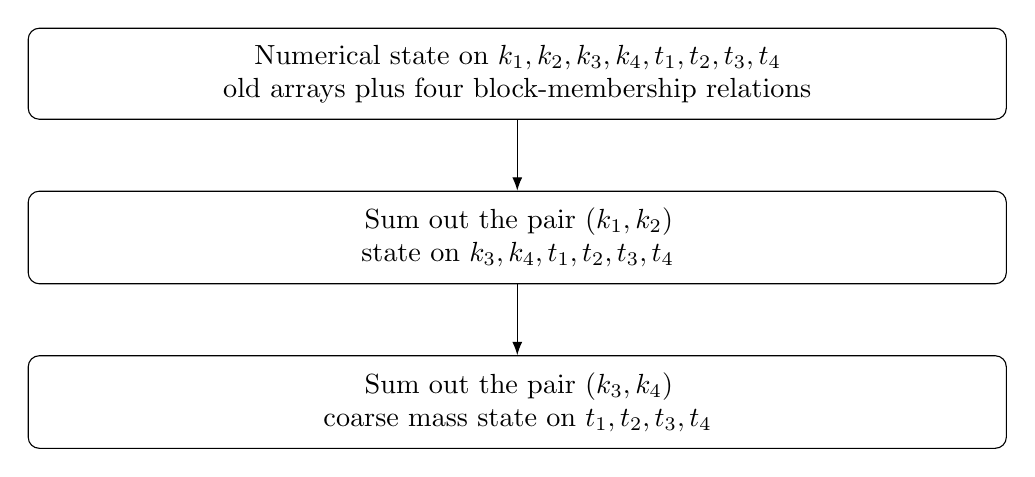
\begin{tikzpicture}[node distance=9mm,>=Latex,
 box/.style={draw,rounded corners,align=center,inner sep=6pt,text width=12cm}]
\node[box] (a) {Numerical state on $k_1,k_2,k_3,k_4,t_1,t_2,t_3,t_4$\\
old arrays plus four block-membership relations};
\node[box,below=of a] (b) {Sum out the pair $(k_1,k_2)$\\
state on $k_3,k_4,t_1,t_2,t_3,t_4$};
\node[box,below=of b] (c) {Sum out the pair $(k_3,k_4)$\\
coarse mass state on $t_1,t_2,t_3,t_4$};
\draw[->] (a)--(b); \draw[->] (b)--(c);
\end{tikzpicture}
\end{center}

\begin{lemma}[Numerical compression]\label{lem:push}
If the old state has $S$ terms and total axis length $M$, compression emits
at most $C_4S$ terms, where
\[
                    C_4=B_8B_7B_6B_5
\]
is a fixed constant. It costs $O(S(M+m)\log(M+m+2))$ arithmetic operations,
with a fixed dimension-dependent constant, and the output uses $O(C_4S(m+1))$
array entries. No product-grid enumeration or density normalization occurs.
\end{lemma}
\begin{proof}
Apply Lemma~\ref{lem:closure} four times to each lifted term. The number
of variables decreases from eight to four. Its original and new axis
domains have total length $M+O(m)$; elimination never introduces another
domain. Each surviving array is indexed by one new variable with at most
$m+1$ entries. This proves the emission, work, and storage bounds.
\end{proof}

\begin{lemma}[Why descendants can use the compressed state]\label{lem:future}
If $g(k)$ is constant on every product of the current blocks, then
\[
                 \sum_k F(k)g(k)=\sum_t(\Push F)(t)g(t).
\]
Every remaining box mask and every subsequent cut is block-aligned.
The same identity therefore remains valid throughout all descendants.
\end{lemma}
\begin{proof}
Group the finite sum by block products. Pull the constant $g$ out of
each inner sum. Every surviving box boundary was used when the blocks
were built. Later cuts are selected only from boundaries of those surviving
boxes, and later absorbed masks come from the same boxes. Thus no
descendant requires a coordinate boundary that has been discarded.
\end{proof}

This is the finite-sum counterpart of conditional expectation, with
\emph{mass} stored directly. A zero-mass cell causes no division by zero.
The anchor may be merged with a neighbouring cell only when all remaining
box masks treat them identically. Once that is true, their summed mass is
all that future computation needs.

\section{The geometric recursion, step by step}\label{sec:recursion}
\subsection{Absorb the easy boxes}
For a box with rank corner $p$, first discard it if $p_i<\ell_i$ for
some axis. For a remaining box, call an axis active when $p_i<u_i$.
There are four cases:
\begin{enumerate}
\item No active axes: the box covers the cell, so return zero uncovered mass.
\item One active axis $i$: multiply $a_i(k_i)$ by $\1[k_i>p_i]$ in every term.
\item Two active axes $i,j$: absorb its complement as a pair condition.
\item Three or four active axes: retain the box as hard.
\end{enumerate}
For a whole group of two-sided boxes on pair $i<j$, build
\[
 f_{ij}(k_i)=\max\{p_j:p_i\ge k_i\},\qquad\max\varnothing=-1.
\]
Its uncovered condition is $k_j\ge f_{ij}(k_i)+1$. This is a nonincreasing
lower-cutoff array. Put each box endpoint in one array position, then take
a suffix maximum; the group costs one scan, not one scan per box.
Multiple slabs on one axis similarly reduce to their largest cutoff.
Absorption does not increase the number of terms.

Unlike a continuous geometric implementation, this version need not shrink
the cell for slabs. Zeroing the corresponding unary entries is sufficient.
Every box retained as hard still has at least three active axes.

\subsection{Two pairs of binary cuts}
The cut axes cycle as
\[
                    (1,2)\ ;\ (3,4)\ ;\ (1,2)\ ;\cdots.
\]
At a cut on axis $i$, a split after index $c$ gives the disjoint children
\[
       [\ell_i,c]\quad\hbox{and}\quad[c+1,u_i].
\]
The answer is the sum of the two child answers. No subtraction or
inclusion--exclusion across children is needed. For the face-count argument,
one may embed index $k$ as the unit cell $[k,k+1)$. A rank cutoff $p_i$
then has its geometric boundary at $p_i+1$. Thus $\ell_i\le p_i<u_i$
correctly identifies an internal boundary, even when $p_i=\ell_i$;
atomic anchor cells require no exception.

For every hard box, form the triples of its active axes. Each triple
represents a one-dimensional face. With positions $0,1,2,3$ measured
cyclically from the current cut axis, assign a triple $J$ weight
\begin{equation}
                      \omega(J)=2^{\sum_{j\in J}\mathrm{pos}(j)/4}.
                                                        \label{eq:weights}
\end{equation}
Let $\Phi$ be the total weight. Each hard box contributes between a
positive constant and another constant, so its number is $\Theta(\Phi)$.
Cut at a weighted median of the cutoff coordinates of those faces whose
triples contain the current axis. Ties go to the same cut; faces at that
cut disappear from both children's active-face lists.

\begin{lemma}[One numerical cut]\label{lem:cut}
With the exact weights in \eqref{eq:weights}, a child has weighted
potential at most $2^{-3/4}\Phi$, after advancing the cyclic axis order.
If no face uses the current axis, advance the axis without splitting;
the same potential decrease holds.
\end{lemma}
\begin{proof}
Split the parent faces into those using the current axis and those not
using it. At most half the weight of the first group survives in either
child. After rotating the axis order, a triple in that group changes its
position sum by $+1$, and its individual weight is multiplied by $2^{1/4}$.
The resulting total is at most $2^{1/4}/2=2^{-3/4}$ times its old total.
For a triple not using the current axis, all three positions decrease by
one, so its weight is multiplied by $2^{-3/4}$. Restricting a cell creates
no new active triples. If the first group is empty, this latter argument
applies to every face without a geometric split.
\end{proof}

\begin{corollary}[One $2+2$ cutting round]\label{cor:round}
After cuts on axes $(1,2)$ followed by $(3,4)$, there are at most $16$
descendants, each with potential at most $\Phi/8$. After $q$ rounds there
are at most $r^4$ descendants of potential at most $\Phi/r^3$, where $r=2^q$.
\end{corollary}
This $16$-versus-$8$ relation is the source of the exponent
$\log_8 16=4/3$. It is not yet a total-work proof: the numerical state
also has to be charged.

\subsection{Purely integer median weights}
The prototype even avoids algebraic constants in selecting a median.
Let $n_0$ be the original number of points and set $A=(n_0+2)^2$.
For a triple with position sum $s\in\{3,4,5,6\}$ use the integer weight
\[
                 W_s=\left\lceil(A^4 2^s)^{1/4}\right\rceil.
\]
Integer square roots compute its floor fourth root exactly; one comparison
decides whether to round upward. Then
\[
       2^{s/4}\le W_s/A\le (1+1/A)2^{s/4}.
\]
A median with these integer weights gives the child-potential bound
$2^{-3/4}(1+1/A)\Phi$. This changes the total cut depth from
$(4/3)\log_2 n_0+O(1)$ by only $O(\log(n_0+2)/A)=O(1)$.
Over the whole path the extra multiplicative factor is bounded by an
absolute constant. Thus rounding does not change the exponent or introduce
an $n^\varepsilon$ loss. The combinatorial counters have $O(\log n_0)$ bits.

\subsection{The block schedule}
At the start of a block, let
\[
 Q=\left\lceil\frac{\text{sum of the current integer face weights}}{A}\right\rceil,
 \qquad
 q=\max\left\{1,\left\lfloor\frac{\log_2 Q}{16}\right\rfloor\right\}.
                                                        \tag{S}
\]
Run $q$ full $2+2$ rounds, hence $4q$ cyclic levels. At each surviving
block leaf, absorb any newly easy boxes, compress onto the remaining hard
grid, and start a new block using its own value of $Q$.
The logarithm in (S) is just an integer bit-length computation.

The reason to use blocks is representation growth. Compressing after every
cut could multiply the number of terms a logarithmic number of times,
which would be a polynomial loss. Schedule (S) reduces the number of
compression generations to $O(\log\log n)$.

\section{Pseudocode that separates the two recursions}\label{sec:pseudo}
\noindent\textbf{Numerical recursion.}
\begin{quote}\ttfamily\small
PairSum(state, i, j):\\
\hspace*{1em}state = SumOut(state, i)\\
\hspace*{1em}return SumOut(state, j)\\[.5em]
Push(state, hard-grid blocks):\\
\hspace*{1em}add four new block-index variables with unit weights\\
\hspace*{1em}add the lower and upper membership bounds for each block\\
\hspace*{1em}state = PairSum(state, old-axis-1, old-axis-2)\\
\hspace*{1em}state = PairSum(state, old-axis-3, old-axis-4)\\
\hspace*{1em}rename the four surviving block-index variables; return state
\end{quote}

\noindent\textbf{Geometric recursion.}
\begin{quote}\ttfamily\small
Solve(state, boxes, cell, axis, levels-left):\\
\hspace*{1em}discard disjoint boxes; absorb all one- and two-sided boxes\\
\hspace*{1em}if a box covers the cell or state is zero: return 0\\
\hspace*{1em}if only a constant number of hard boxes remain:\\
\hspace*{2em}return the numerical base case\\
\hspace*{1em}if levels-left is zero:\\
\hspace*{2em}build blocks from all remaining hard-box cutoffs\\
\hspace*{2em}state = Push(state, blocks); relabel boxes and cell\\
\hspace*{2em}levels-left = 4q from schedule (S)\\
\hspace*{1em}find the weighted median on the current axis\\
\hspace*{1em}if there is no cut candidate:\\
\hspace*{2em}recurse on the same cell, next axis, one fewer level\\
\hspace*{1em}else:\\
\hspace*{2em}split after the median; recurse on both children\\
\hspace*{2em}return the sum of their answers
\end{quote}
The first block is initialized by (S). Each axis advance, including a
skip, consumes one level. Four advances return to the original axis order.

For a base case of at most $b$ hard boxes, where $b$ is a fixed constant,
expand $\prod_{p\in B}(1-\1[k\le p])$ over its $2^b$ subsets.
Each subset restricts the upper endpoint of a rectangle. Apply the two
pair sums to that restricted rectangle and take the alternating sum.
This is constant-size inclusion--exclusion; it is not exponential in $n$.
The prototype defaults to $b=2$ and uses $b=1$ in several stress tests.

\section{Correctness and the complete work bound}\label{sec:complexity}
\subsection{Correctness}
\begin{proof}[Correctness part of Theorem~\ref{thm:main}]
Lemma~\ref{lem:discrete} gives the exact initial numerical problem.
Absorption multiplies the state by the complement of each removed box,
so it preserves \eqref{eq:invariant}. A split partitions the index cell
into two disjoint sets. Every numerical elimination sums one index
exactly, including ties and zero-index anchor cells.
Lemmas~\ref{lem:push} and~\ref{lem:future} justify compression and its
future reuse. Finally the base case is a finite inclusion--exclusion
identity evaluated by exact pair sums. These facts prove correctness
inductively; \eqref{eq:answer} recovers the covered mass.
\end{proof}

\subsection{One block, with term growth included}
At a block entry let $N$ be its weighted hard-face potential and let
$S$ be its number of terms. Apart from the first block, the axis-list
length is $O(N)$ because the previous compression used only surviving
hard cutoffs. The first block has $O(n)$ entries and is charged at root size.

For sufficiently large $N$, schedule (S) gives
\[
             r=2^q=\Theta(N^{1/16}),\qquad
             r^4=O(N^{1/4}).
\]
There are $O(r^4)$ nodes and leaves within a block. Absorptions, cuts,
copies, and the compression at each block leaf each cost at most
$O(SN\log^{O(1)}(N+2))$, with a fixed constant accounting for the
elimination kernel. Early numerical base cases satisfy the same charge.
Thus the entire block costs
\begin{equation}
                    O(SN^{5/4}\log^{O(1)}(N+2)).     \label{eq:blockcost}
\end{equation}
Each child block has potential at most $c_0N^{13/16}$ and at most
$C_4S$ terms. The constant $c_0$ includes integer rounding of the block
length and the bounded median-weight approximation factor.

Writing $T(N,S)$ for all remaining work gives the transparent recurrence
\begin{equation}
 \boxed{\displaystyle
 T(N,S)\le c_1N^{1/4}T(c_0N^{13/16},C_4S)
                 +c_2SN^{5/4}\log^{c_3}(N+2).}
                                                        \label{eq:recurrence}
\end{equation}
All constants are independent of $N$ and $S$. For bounded $N$, only a
bounded number of further geometric levels is possible, and the same
claim holds with a fixed-dimensional constant base cost.

\subsection{Solving the recurrence explicitly}
Put $\beta=13/16$. At macro-depth $g$, the worst-case child size is
$N_g\le c_4N^{\beta^g}$. Consequently only $O(\log\log(N+2))$
macro-generations occur before reaching a fixed constant size. The term
count along any path is bounded by
\begin{equation}
                     S_g\le C_4^gS=S\log^{O(1)}(N+2).
                                                        \label{eq:terms}
\end{equation}
No unproved canonical-merging bound is used here.

The number of nodes at macro-depth $g$ is at most
\[
 c_5^g\prod_{h<g}(N^{\beta^h})^{1/4}
       =c_5^gN^{\frac43(1-\beta^g)}.
\]
Multiplying this by the per-node charge $S_gN_g^{5/4}$ gives, apart from
polylogarithmic factors,
\[
 S N^{\frac43(1-\beta^g)+\frac54\beta^g}
       =S N^{\frac43-\frac1{12}\beta^g}
       \le S N^{4/3}.
\]
The constants raised to $g$ and the number of macro-levels are
polylogarithmic. Summing proves $T(N,S)=\wtO(SN^{4/3})$.
Initially $S=1$ and $N=O(n)$, completing Theorem~\ref{thm:main}.

This proof tolerates very large dimension-dependent emission constants.
It also explains why counting leaves alone, or observing that empirical
term counts stayed small, would be insufficient.

\section{A worked four-point example}\label{sec:example}
Consider
\[
\begin{split}
 p_1&=(1,4,3,2),\qquad p_2=(2,3,4,1),\\
 p_3&=(3,2,1,4),\qquad p_4=(4,1,2,3).
\end{split}
\]
Each axis list is $(0,1,2,3,4)$. The hypervolume masses are
$(0,1,1,1,1)$; the magnitude masses are
$(1,\tfrac12,\tfrac12,\tfrac12,\tfrac12)$.
Each point has exactly three active axes at the root.

On the first axis the cut candidates are $1,2,3$, with weights
$2^{5/4},2^{4/4},2^{3/4}$ respectively. The weighted median is $2$.
The integer weights used by the prototype select the same cut.
The left index cell has $k_1\in[0,2]$, and the right has $k_1\in[3,4]$.

In the left child, $p_2$ is now two-sided on axes $(2,4)$, and $p_3$
is two-sided on axes $(2,3)$. Their complements enter the numerical state
as two pair predicates. Only $p_1,p_4$ remain hard.
In the right child, $p_1,p_2$ are disjoint and disappear; $p_3,p_4$ remain.
With base threshold two, both children are already base cases.

To illustrate compression at the left child, its surviving hard cutoffs
would give these index blocks:
\[
\begin{array}{c|l}
\text{axis}&\text{blocks}\\\hline
1 &[0,1],\ [2,2]\\
2 &[0,1],\ [2,4]\\
3 &[0,2],\ [3,3],\ [4,4]\\
4 &[0,2],\ [3,3],\ [4,4]
\end{array}
\]
The constructor computes their mass state through the eight-variable
pairwise elimination; it does not visit the $2\cdot2\cdot3\cdot3=36$
block products. This early compression is explanatory, not required by
the default block schedule.

The complete numerical computation gives
\[
                   \HV_4(P)=69,\qquad
                   \Mag(D(P))=\frac{765}{16}.
\]
Both are verified independently by inclusion--exclusion over the four
original boxes. The geometry and cutoff comparisons are identical in
the two runs; only the initial axis masses change.

\section{Magnitude and hypervolume in both directions}
For nonempty $P$, the product measure of one anchored box is
$\prod_i(1+p_i/2)$. Coordinatewise minimum describes intersections of
anchored boxes and commutes with the affine map $p\mapsto\1+p/2$.
Finite inclusion--exclusion therefore proves
\begin{equation}
              \Mag(D(P))=\HV_4(\{\1+p/2:p\in P\}).    \label{eq:affine}
\end{equation}
The equality also holds for empty input when its union measure is zero.

Conversely, if every coordinate of every HV corner $q$ is at least one,
\[
                    \HV_4(Q)=\Mag(D(\{2(q-\1):q\in Q\})).
\]
For arbitrary strictly positive HV corners, choose a common scale
$s$ with $sq_i\ge1$ and use
\[
                    \HV_4(Q)=s^{-4}
                    \Mag(D(\{2(sq-\1):q\in Q\})).
\]
Boxes with a zero coordinate can first be removed for this inverse HV
reduction because their four-dimensional volume is zero. They must not
be removed in a magnitude computation.

The numerical engine can thus compute magnitude either directly through
its atomic product masses or by the affine HV transform. The direct
route is useful for testing endpoint correctness and for keeping the
algebra of product measures visible. Neither direction improves the
exponent by itself.

\section{Relation to the supplied repositories}\label{sec:repos}
The following sources were inspected at pinned revisions on 4 October 2026:
\begin{itemize}
\item \texttt{FastHVChan}, commit \texttt{08539aa99e94}, including
      \texttt{chan\_orthant\_dby3.py} and the accompanying paper~\cite{fastrepo}.
\item \texttt{HV4DMagnitude}, commit \texttt{0c668e765202}, including
      \texttt{solver.py}, the audit, the closed four-dimensional report,
      and the pair-elimination report~\cite{magrepo,magreport}.
\item Its \texttt{HV468DMagnitude} code and complexity/audit reports,
      especially the distinction between static elimination and the
      $2d$-variable compression problem~\cite{higherrepo}.
\end{itemize}

The present construction is a discrete specialization of the same
active-bound elimination idea. It does not claim a new hypervolume
exponent or a new general elimination principle. Its useful changes
are the numerical representation and the explicit closure/scheduling proof.

\begin{center}\small
\begin{tabular}{@{}p{.43\linewidth}p{.50\linewidth}@{}}
\toprule
Continuous implementation ingredient&Finite numerical replacement\\\midrule
Step-function evaluation and inversion&Integer cutoff arrays and binary search\\
Antiderivative or threshold integral&Prefix sums of numerical unary weights\\
Decorated endpoints and anchor cases&One anchor cell; integer inclusive bounds\\
Compact finite-turn inverse&Keep the four monotone slots separate\\
Average density on a hard grid&Mass pushed to blocks, with no division\\
Symbolic breakpoint proliferation&Fixed one-dimensional index domains\\
Assumed small held state&Raw emission constant and $O(\log\log n)$ generations\\
\bottomrule
\end{tabular}
\end{center}

The supplied \texttt{solver.py} is explicitly a correctness-oriented
prefix-normal-form solver. It sends its live orthants into the children
and rebuilds the easy state; it does not perform periodic compression.
Our prototype discards absorbed boxes and carries their numerical mass
state forward. Its worst-case proof charges compression explicitly.
We do not infer a time bound from compression failing to trigger in
particular experiments.

There is still a short structural term constructor: it enumerates winning
bounds and installs array comparisons. Calling this implementation
``numerical'' means that all stored data and all evaluations are finite
arrays and numbers. It does not mean that the necessary case distinctions
have disappeared or that there is a single fixed six-number summary.

\section{Implementation and verification}\label{sec:validation}
The accompanying standard-library Python implementation is
\texttt{numerical\_chan4.py}; its independent verifier is
\texttt{verify\_numerical\_chan4.py}. The implementation is under 400 lines,
including documentation and counters. Its main entry points are:
\begin{quote}\ttfamily\small
solver = NumericalChan4()\\
hv = solver.compute(points)\\
mag = solver.compute(points, magnitude=True)
\end{quote}
Integer or \texttt{Fraction} coordinates give exact rational arithmetic.
Float input gives the floating-point evaluation of the same algorithm.
Signed terms can cancel; the exact-arithmetic theorem is not a promise
of a small floating-point error. The prototype uses exact-key merging and
normalizes nonzero unary factors for better reuse. These optimizations are
not needed for the raw-emission proof.

The completed verification has the following scope:
\begin{center}\small
\begin{tabular}{@{}p{.72\linewidth}r@{}}
\toprule
Check&Count\\\midrule
Strict/non-strict bound-comparison grid entries&5760\\
One-variable elimination output entries&1184\\
Complete finite sums, including signed weights&71\\
First-compression cell masses&32\\
Second compression after a new aligned mask&2\\
End-to-end HV/magnitude instances, exact inclusion--exclusion&54\\
Forced deep recursion instances&2\\
Magnitude--HV affine equivalence instances&6\\
Geometric face-weight contraction checks&358\\
Independent FastHVChan cross-checks&4\\\bottomrule
\end{tabular}
\end{center}
The predicate tests exercise increasing and decreasing cutoffs, both
inequality senses, ties, reversed argument order, and an alternating
same-variable filter. Static numerical elimination is checked up to eight
variables. Compression is tested at the full eight variables needed in 4D.
The geometric contraction checks use floating-point evaluation only for
the fixed algebraic face weights, with a tolerance; the measure and
elimination comparisons use exact arithmetic.

A reproducible twelve-point instance shows the effect of scheduling:
\begin{center}\small
\begin{tabular}{@{}llrrr@{}}
\toprule
Schedule&Measure&Generations&Compressions&Peak terms\\\midrule
Default block rule&HV&1&1&8\\
Default block rule&Magnitude&1&1&24\\
One-level stress rule&HV&4&11&451\\
One-level stress rule&Magnitude&4&11&473\\\bottomrule
\end{tabular}
\end{center}
``Generations'' is the maximum along a path; ``compressions'' counts all
branches. Both schedules give $1492$ for HV and $1215/4$ for magnitude
on this instance. The one-level override is a closure stress test and is
\emph{not} the schedule covered by the asymptotic theorem.
These small tests establish implementation checks, not an empirical
measurement of the $4/3$ exponent or a speed advantage over existing code.

\section{Numba implementation and measured comparison}
The directory \texttt{NumericalChanHV4D} also supplies
\texttt{numerical\_chan4\_numba.py}, a four-dimensional entry point to
the shared \texttt{float64} engine in \texttt{NumericalChanHVND}.
The shared engine compiles numerical array scans, prefix sums, cutoff
searches, normalization, and suffix masks with Numba. Geometric recursion
and structural term construction remain Python; it is a hybrid backend.
The exact standard-library implementation remains independently usable.
Neither fastmath nor parallel execution is enabled.

The reproducible benchmark compares the numerical Python and Numba
backends with the repository's unmodified Python implementations of Chan
Section~4.2 ($d/3$) and Section~2 ($d/2$). The baseline commit is
\texttt{08539aa99e94}; neither baseline uses Numba. All timed inputs are
floating point. Dominance prefiltering is disabled, and input preprocessing
and coordinate transforms are included. For magnitude, the references use
the affine HV transformation.

Each entry below is the median of three calls after one untimed first call.
Workers run sequentially. A 35-second limit covers the entire worker,
including startup, its first call and all repeats; ``timeout'' is not a
per-call runtime. Raw repeats and first-call times are in the accompanying
JSON/CSV. No ratio is assigned to a timeout.

\begin{center}\small
\begin{tabular}{@{}lrrrr@{}}
\toprule
Case&Numerical Python&Numba&Chan 4.2&Chan 2\\
\midrule
sphere, 12, HV&0.028069&0.041134&0.012223&0.0017601\\
sphere, 12, Mag&0.028301&0.043302&0.0126&0.0019805\\
sphere, 24, HV&1.4637&2.3398&0.027249&0.0054424\\
sphere, 48, HV&timeout&timeout&0.10325&0.018492\\
grid, 12, HV&0.0046516&0.0064536&0.0030063&0.0005476\\
grid, 12, Mag&0.004033&0.006346&0.0034868&0.000561\\
grid, 24, HV&0.045366&0.076442&0.0065916&0.001393\\
grid, 48, HV&0.074685&0.1358&0.0018386&0.0009735\\
\bottomrule
\end{tabular}
\end{center}
All times are seconds. The ND overview uses spherical, mutually
nondominated fronts; the full data additionally includes tied-grid inputs
and magnitude evaluations. These small cases do not measure asymptotic exponents.

For completed matched ordinary-HV cases in 4D, the median ratio Numba numerical / Python numerical was 1.60x (5 cases). The median ratio Numba numerical / the repository's Python Section~4.2 implementation was 11.60x (5 cases). Ratios above one mean the Numba version was slower. These are medians of per-case ratios for this small benchmark set. They do not support a practical speedup claim for this four-dimensional implementation.

Across completed comparisons the maximum scaled disagreement was $3.31\times10^{-16}$, where scaling divides by $\max(1,|\text{reference value}|)$. This is an observed check, not a uniform error bound.

Fresh-cache first-use probes (module imports excluded) gave:
\begin{center}\small
\begin{tabular}{@{}crr@{}}\toprule
Dimension&First use (s)&Second use (s)\\\midrule
2&2.5352&9.72e-05\\
3&2.496&0.0001481\\
4&1.9391&0.0030841\\
\bottomrule
\end{tabular}
\end{center}
The first call includes both compilation and computation; it is not pure compiler time.

Environment: CPython 3.12.14, NumPy 2.5.3, Numba 0.68.0, Windows.


\section{What extends to dimensions six and eight}
The numerical term class and its four slots per pair are dimension
independent. In dimension $d$, compression introduces $2d$ variables
and eliminates the old $d$, in pairs when $d$ is even. The raw constant is
\[
                   C_d=\prod_{p=d+1}^{2d}B_p.
\]
It can be very large, but is independent of the number of input points.
For $d=6,8$, the compression dimensions are respectively $12,16$.

The geometric potential uses active triples exactly as before, now with
weights $2^{\sum\mathrm{pos}/d}$. A cyclic level decreases potential by
$2^{-3/d}$; a full $d$-axis round creates at most $2^d$ descendants and
decreases potential by a factor eight. Taking approximately
$\tfrac14\log_2N$ levels per locally chosen block gives
\[
 T_d(N,S)\le O(N^{1/4})
       T_d\bigl(O(N^{1-3/(4d)}),C_dS\bigr)
                 +\wtO_d(SN^{5/4}).
\]
Since $5/4<d/3$ for $d\ge4$, the same analysis gives
$\wtO_d(n^{d/3})$: $\wtO(n^2)$ in six dimensions and
$\wtO(n^{8/3})$ in eight dimensions. This describes the mathematical
extension. The standalone reference solver in this directory is
four-dimensional. The companion directory \texttt{NumericalChanHVND}
now implements and tests every dimension from two through ten, including
12-, 16-, and 20-variable compression. Its own report distinguishes small
structured validation from practical performance on large coupled inputs.

\section{The resulting algorithmic target}
The requested $\wtO(n^{4/3})$ numerical formulation is obtained without
the unproved global batching step from the earlier faster-algorithm
investigation. Its complexity follows from Chan's geometric cuts plus a
proved finite-array compression and a schedule that explicitly pays for
term growth.

The reusable core is small: four monotone slots per pair, one prefix-sum
eliminator, and block-mass pushforward. The geometric recursion is binary,
organized into the coordinate pairs $(1,2)$ and $(3,4)$. Further practical
work can specialize these fixed operations or compile their arrays, while
keeping the same correctness and complexity argument.

\begin{thebibliography}{9}
\raggedright
\bibitem{chan}
T. M. Chan. \emph{Klee's Measure Problem Made Easy}.
Proceedings of FOCS 2013, pp. 410--419.
DOI: 10.1109/FOCS.2013.51.
Author's August 2013 version, Sections 4.1--4.2:
\url{https://tmc.web.engr.illinois.edu/easyklee8_13.pdf}.

\bibitem{emmerich}
M. T. M. Emmerich. \emph{The Magnitude of Dominated Sets: A Pareto Compliant
Indicator Grounded in Metric Geometry}. arXiv:2604.18147, 2026.
\url{https://arxiv.org/abs/2604.18147}.

\bibitem{fastrepo}
M. Emmerich and collaborators. \emph{FastHVChan}: source code and
implementation report. Repository snapshot \texttt{08539aa99e94},
accessed 4 October 2026.
\url{https://github.com/emmerichmtm/FastHVChan}.

\bibitem{magrepo}
M. Emmerich and collaborators. \emph{HV4DMagnitude}: numerical prefix
formulation, audits, and implementation. Repository snapshot
\texttt{0c668e765202}, accessed 4 October 2026.
\url{https://github.com/emmerichmtm/HV4DMagnitude}.

\bibitem{magreport}
M. T. M. Emmerich. \emph{Pair-Elimination and Product-Measure Simplification
of Chan's Fixed-Dimensional Hypervolume Algorithm}. Working report,
\texttt{paper/magnitude\_chan\_pair\_elimination\_report.tex}, in
the \texttt{HV4DMagnitude} snapshot cited above. Also inspected:
\texttt{paper/magnitude\_chan4\_report\_closed.tex}.

\bibitem{higherrepo}
\emph{HV468DMagnitude}: pair-elimination implementation and audit material,
including \texttt{PAIR\_ELIMINATION\_COMPLEXITY.md} and
\texttt{AUDIT\_RESPONSE.md}, in the \texttt{HV4DMagnitude} snapshot above.
\url{https://github.com/emmerichmtm/HV4DMagnitude/tree/main/HV468DMagnitude}.
\end{thebibliography}
\end{document}
